\documentclass{article}
\usepackage[utf8]{inputenc}
\setlength{\parindent}{0em}
\setlength{\parskip}{1em}
\usepackage{listings}
\usepackage{pdfpages}


\title{MSc Scientific Computing Dissertation\\ARM Cluster Linpack Benchmarks}
\author{John Duffy}
\date{August 2020}

\begin{document}

\maketitle



\section{Introduction}

\begin{verbatim}
https://github.com/johnduffymsc/picluster
\end{verbatim}

\subsection{Aims}

\subsubsection{Investigate Maximum Achievable Linpack Benchmark}

Efficiency... achieved vs theoretical maximum

\subsubsection{Investigate Gflops/Watt}

Green500 ranking...

\subsubsection{Overview of Competitive Available Gflops/£}

Buy lots of Pi's, or buy a bigger machine...

Plot Gflops vs £...



\section{Raspberry Pi 4 Model B}

\subsection{Description}

Photo...

Description...

Highlights...

Limitations...

Reference data sheet in Appendix...



\subsection{Theoretical Maximum Performance (Gflop/s)}

The Raspberry Pi 4 Model B uses the Broadcom BCM2711 System on a Chip (Soc).

Block diagram from Cortex-A72 Software Optimisation Guide

4 cores

1.5 GHz

128 bit SIMD

4 GB memory (our chosen model)

Caches...

Pipeline...

Simplistically, ...

This ignores instructions pipelining benefits...



\section{Pi Cluster}

Photo...

Description...

Ubuntu 20.04 LTS 64-bit Preinstalled Server...

Reference Appendix A for detailed build instructions...

Limitations...

Software/update management...

Next PXE/NFS boot...

Cluster management tools

BLAS libraries...

BLAS library management... update-alternatives --config libblas.so.3-aarch64-linux-gnu

picluster/tools... appendix ?... use from node1...



\section{High-Performance Linpack (HPL) Benchmark}

Reference Paper...

https://www.netlib.org/benchmark/hpl/...

Describe algorithm...

Terminology $R_{peak}$, $R_{max}$..., problem size...

Describe methodology for determining main parameters NB, N, P and Q...

N formula...

Reference http://hpl-calculator.sourceforge.net



\subsection{Building and Installing HPL}

See Appendix...



\subsection{HPL.dat}

Describe HPL.dat parameters...

\lstinputlisting[frame=single, caption=Example HPL.dat]{files/HPL.dat}

A detailed description of each line of this file is ...

\subsection{HPL.out}

Describe HPL.out...

It is very easy to use \verb grep to find the lines in HPL.out containing the results. And to then conduct a general numeric sort, first by P and then by Gflops, to find Rmax for each P and Q pair, squeezing repeated white space down to a single space for readability.

\begin{verbatim}
grep WR HPL.out | sort -g -k 4 -k 7 | tr -s ' ' > HPL.out.sorted
\end{verbatim}

\lstinputlisting[frame=single, caption=Example HPL.out.sorted]{files/HPL.out.sorted}




\subsection{Running xhpl}

To run xhpl using the serial version of OpenBLAS...

~/picluster/tools/picluster-set-libblas-openblas-serial

cd ~/picluster/hpl/hpl-2.3/bin/serial

mpirun -host node1:4 -np 4 xhpl



To run xhpl using the OpenMP version of OpenBLAS...

~/picluster/tools/picluster-set-libblas-openblas-openmp

export OMPNUMTHREADS=4 TODO: SET GLOBALLY AT INSTALLATION

export BLISNUMTHREADS=4 TODO: SET GLOBALLY AT INSTALLATION

cd ~/picluster/hpl/hpl-2.3/bin/serial



\section{OpenMPI}

What is OpenMPI...



\section{OpenMP}

What is OpenMP...



\section{OpenMPI Baseline Benchmarks}

Ubuntu 20.04 LTS 64-bit packages, without any tweaks...

1 core... a single ARM Cortex-A72 core...

1 node... a single Raspberry Pi 4 Model B, 4 x ARM Cortex-A72 cores...

Linpack performance scales with problem size... REFERENCE

80\% of memory a good initial guess... FAQ REFERENCE...


Methodology...

1 core... to investigate single core performance... caveats... use 1GB of memory...

1 node... to investigate inter-core performance...

2 nodes... to investigate inter-core and inter-node performance...

1..8 nodes ... to investigate over scaling of performance with node count... with optimal N, NB, P and Q parameters determined from 2 node investigation... caveats...



\subsection{1 Core Baseline Benchmark}

Problem size restricted to 80\% of 1GB...

NB 32 to 256 in increments of 8...

\begin{center}
	\begin{tabular}{ |c|c|c|c|c|c|c|c|c|c| } 
		\hline
		NB & N & NB & N & NB & N & NB & N & NB & N \\ 
		\hline
		32 & 9248 &  80 & 9200 & 128 & 9216 & 176 & 9152 & 224 & 9184 \\ 
		40 & 9240 &  88 & 9240 & 136 & 9248 & 184 & 9200 & 232 & 9048 \\ 
 		48 & 9264 &  96 & 9216 & 144 & 9216 & 192 & 9216 & 240 & 9120 \\
		56 & 9240 & 104 & 9256 & 152 & 9120 & 200 & 9200 & 248 & 9176 \\ 
 		64 & 9216 & 112 & 9184 & 160 & 9120 & 208 & 9152 & 256 & 9216 \\
		72 & 9216 & 120 & 9240 & 168 & 9240 & 216 & 9072 &   - &    - \\ 
 		\hline
	\end{tabular}
\end{center}

1x1

%\begin{verbatim}[frame=single, backgroundcolor=\color{yellow},basicstyle=\ttfamily]
\begin{verbatim}
    $ mpirun -np 1 xhpl
\end{verbatim}

mpirun does bind to core by default for $np \leq 2$

\begin{figure}
	\centering	
	\includegraphics[width=1.0\textwidth]{../gflops_vs_nb_1_core_80_percent_memory.pdf}
	\caption{1 Core $R_{max}$ vs NB using 80\% of 1GB memory.}
\end{figure}

4 x 4.7527e+00 = 19 Gflops

Explain...

Cache misses from peak...

A single core is capable of achieving maximum theoretical performance... CAVEATS whole L2 cache, whole node 4 GB memory, although problem size limited to 80\% of 1 GB...  


\subsection{1 Node Benchmark}

1x4

\begin{center}
	\begin{tabular}{ |c|c|c|c|c|c|c|c|c|c| } 
		\hline
		NB & N & NB & N & NB & N & NB & N & NB & N \\ 
		\hline
		32 & 18528 &  80 & 18480 & 128 & 18432 & 176 & 18480 & 224 & 18368 \\ 
		40 & 18520 &  88 & 18480 & 136 & 18496 & 184 & 18400 & 232 & 18328 \\ 
 		48 & 18528 &  96 & 18528 & 144 & 18432 & 192 & 18432 & 240 & 18480 \\
		56 & 18536 & 104 & 18512 & 152 & 18392 & 200 & 18400 & 248 & 18352 \\ 
 		64 & 18496 & 112 & 18480 & 160 & 18400 & 208 & 18512 & 256 & 18432 \\
		72 & 18504 & 120 & 18480 & 168 & 18480 & 216 & 18360 &   - &     - \\ 
 		\hline
	\end{tabular}
\end{center}

%\lstset{frameround=tttt}
\begin{lstlisting}[frame=single]
mpirun -np 4 xhpl
\end{lstlisting}

mpirun does bind to socket by default for $np \geq 2$

\begin{figure}
	\centering	
	\includegraphics[width=1.0\textwidth]{../gflops_vs_nb_1_node_80_percent_memory.pdf}
	\caption{1 Node $R_{max}$ vs NB using 80\% of 4GB memory.}
\end{figure}



\subsection{2 Node Baseline Benchmark}

P1 x Q8

P2 x Q4

\begin{center}
	\begin{tabular}{ |c|c|c|c|c|c|c|c|c|c| } 
		\hline
		NB & N & NB & N & NB & N & NB & N & NB & N \\ 
		\hline
		32 & 26208 &   80 & 26160 & 128 & 26112 & 176 & 26048 & 224 & 26208 \\ 
		40 & 26200 &   88 & 26136 & 136 & 26112 & 184 & 26128 & 232 & 25984 \\ 
 		48 & 26208 &   96 & 26208 & 144 & 26208 & 192 & 26112 & 240 & 26160 \\
		56 & 26208 & 104 & 26208 & 152 & 26144 & 200 & 26200 & 248 & 26040 \\ 
 		64 & 26176 & 112 & 26208 & 160 & 26080 & 208 & 26208 & 256 & 26112 \\
		72 & 26208 & 120 & 26160 & 168 & 26208 & 216 & 26136 &     - &         - \\ 
 		\hline
	\end{tabular}
\end{center}


%\begin{figure}
%	\centering	
%	\includegraphics[width=1.0\textwidth]{../gflops_vs_nb_2_node_80_percent_memory.pdf}
%	\caption{2 Node $R_{max}$ vs NB using 80\% memory.}
%\end{figure}


\subsection{8 Node Baseline Benchmark}

1x32
2x16
4x8

%\begin{figure}
%	\centering	
%	\includegraphics[width=1.0\textwidth]{pdfs/gflops_vs_nodes_80_percent_memory.pdf}
%	\caption{The maximum Gflops achieved using 80 of total available memory.}
%\end{figure}



\subsection{Observations}

Best NB...

PxQ discussion... 1x8 vs 2x4... ethernet comment...

Iperf...

htop...

top...

perf...

cache misses...

software interrupts...

Suggests... improve network efficiency?



%
% OLD STUFF FROM HERE UP TO APPENDICES- WEED!
%



% SUBSECTION
\subsection{Baseline Benchmark}
As per software installation from Ubuntu Server 20.04 LTS.

OpenBLAS

OpenMP

OpenMPI

HPL-2.3 compiled with Make.rpi4.baseline

NB = 128 (mid-range guess; to be tuned based on L1 cache size)

N for 80\% efficiency (from tool)

Recommended: P$\times$Q as square as possible, with Q $>$ P

4 cores per node
1.5 GHz clock speed
4 GB memory per node
2 instructions per cycle (estimated as NEON is 128 bits)

From tool:

%\begin{center}
%\begin{tabular}{ |c|c|c|c|c|c| } 
%   \hline
%    Nodes & P & Q & NB & N & R_{max}\\
%    1 & 1 & 4 & 128 & 18,432 & 10.0 \\ 
%    2 & 2 & 4 & 128 & 26,112 & 20.0 \\ 
%   3 & 2 & 6 & 128 & 32,000 & 30.0 \\ 
%    4 & 2 & 8 & 128 & 36,992 & 40.0 \\ 
%   5 & 2 & 5 & 128 & 41,344 & 50.0 \\ 
%    6 & 4 & 6 & 128 & 45,312 & 60.0 \\ 
%    7 & 4 & 7 & 128 & 49,024 & 70.0 \\ 
%    8 & 4 & 8 & 128 & 52,352 & 80.0 \\ 
%    \hline
%\end{tabular}
%\end{center}

Run:

\begin{verbatim}
mpirun -host node1:4 -np 4 xhpl
mpirun -host node1:4,node2:4 -np 8 xhpl
mpirun -host node1:4,node2:4,node3:4 -np 12 xhpl
etc
\end{verbatim}

TABLE RESULTS - Gflops vs node count, time vs node count
GRAPH RESULTS - Gflops vs node count, time vs node count

Discussion...

NB size...

P\\Q Ratio...

Node number scaling...


% SUBSECTION
\subsection{OpenMPI without OpenMP}

Describe processor grid layout.

hosts-with-slots file.

% SUBSECTION
\subsection{OpenMPI with OpenMP}

Describe processor grid layout.

hosts-no-slots file.

%
% SECTION
%
\section{Performance Optimisation}


% SUBSECTION
\subsection{Methodology}
1. Measure

2. Study results and propose theory

3. Change something based on 2.

4. Measure

5. Repeat steps 1 - 4


%
% SECTION
%
\section{Build Kernel with Jumbo Frames Support}

Standard MTU is 1500 bytes...

Maximum payload size is 1472 bytes...

NB of 184 (x 8 bytes for Double Precision) = 1472 bytes...

NB $>$ 184 $=>$ packet fragmentation $=>$ reduced network efficiency...

This causes drop of in performance???...

Max MTU on Raspberry Pi 4 Model B is set at build time to 1500...

Not configurable above 1500...

TODO: EXAMPLE OF ERROR MSG...

Need to build the kernel with higher MTU...


Make source packages available...

\begin{verbatim}
    sudo touch /etc/apt/sources.list.d/picluster.list
    sudo vim /etc/apt/sources.list.d/picluster.list...
        deb-src http://archive.ubuntu.com/ubuntu focal main
        deb-src http://archive.ubuntu.com/ubuntu focal-updates main
    sudo apt update
\end{verbatim}

Create a kernel build directory with the correct access permissions to prevent source download warnings. 

\begin{verbatim}
    mkdir kernel
    sudo chown _apt:root kernel
    cd kernel
\end{verbatim}

Install the kernel build dependencies...

\begin{verbatim}
    sudo apt-get build-dep linux linux-image-$(uname -r)
\end{verbatim}

Download the kernel source...

\begin{verbatim}
    sudo apt-get source linux-image-$(uname -r)
\end{verbatim}

Make the required changes to the source... as per REFERENCE

\begin{verbatim}
    cd linux-raspi-5.4.0 

    sudo vim include/linux/if_vlan.h...
        #define VLAN_ETH_DATA_LEN   9000
        #define VLAN_ETH_FRAME_LEN  9018
    
    sudo vim include/uapi/linux/if_ether.h...
        #define ETH_DATA_LEN        9000
        #define ETH_FRAME_LEN       9014
    
    sudo vim drivers/net/ethernet/broadcom/genet/bcmgenet.c...
        #define RX_BUF_LENGTH       10240
\end{verbatim}

Add a Jumbo Frames identifier, "+jf", to the new kernel name...

\begin{verbatim}
    sudo vim debian.raspi/changelog...
        linux (5.4.0-1013.13+jf) focal; urgency=medium
        
\end{verbatim}

Build the kernel...

\begin{verbatim}
    sudo LANG=C fakeroot debian/rules clean
    sudo LANG=C fakeroot debian/rules binary
\end{verbatim}

Install the new kernel...

\begin{verbatim}
    sudo sudo dpkg -i linux*5.4????????.deb
\end{verbatim}

%TODO: SHOW NEW DEFAULT MTU SETTING = 9000

%TODO: EXAMPLES OF ABILITY TO SET MTU ABOVE 1500 UP TO 9000

%TODO: WARNING ABOUT ROUTER/SWITCH & OTHER NODE MTU's


%
% SECTION
%
\section{Single Core Optimisation}

% SUBSECTION
\subsection{Block Size Optimisation}

The block size, NB tuning parameter, is used for matrix calculations and also for network transport.

The most efficient block size is related to the L1 cache size. Describe...


%
% SECTION
%
\section{Single Node Optimisation}


%
% SECTION
%
\section{Cluster Optimisation}




% SUBSECTION
\subsection{Recompile HPL for Cortex-A72}

Block size!

RESULTS

% SUBSECTION
\subsection{Recompile OpenBLAS with OpenMP Support}

As advised by the DebianScience/LinearAlgebraLibraries, OpenBLAS should be recompiled from source for best performance.??? See comflicting statement below.

The Ubuntu/Debian OpenBLAS package is an ARM64 multi-architecture build of OpenBLAS which includes the ARM Cortex-A72. As stated in the README.Debian, performance improvements will be minimal by compiling from source.

However, Ubuntu/Debian build does not include support for OpenMP. So, to test the combination of OpenMPI/OpenMP it is necessary to recompile OpenBLAS from source.

To download the same version of OpenBLAS as Ubuntu 20.04 Server LTS (v0.3.8):

\begin{verbatim}
    cd ~/phas0077/downloads
    wget https://github.com/xianyi/OpenBLAS/archive/v0.3.8.zip -O OpenBLAS-0.3.8.zip
    cp OpenBLAS-0.3.8.zip ~/phas0077/projects
    cd ~/phas0077/projects
    unzip OpenBLAS-0.3.8.zip
    rm OpenBLAS-0.3.8.zip
    cd OpenBLAS-0.3.8
    cp Makefile.rule Makefile.rule.original
    vim Makefile.rule
    make
    make install
    make clean
\end{verbatim}

PROCESSOR AFFINITY - include later.

Need to edit 'Makefile.rule'.

The file 'Makefile.arm64' already has the following so there is no need to add specific architecture flags to 'Makefile.rule'.

\begin{verbatim}
    ifeq ($(CORE), CORTEXA72)
    CCOMMON_OPT += -march=armv8-a -mtune=cortex-a72
    FCOMMON_OPT += -march=armv8-a -mtune=cortex-a72
    endif
\end{verbatim}



Block size!

TODO: Read DebianScience howto recompile/package

TODO: Check ARM gcc options; -mune, -march for ARM Cortex-A72
USE LD\_PRELOAD trick to use recompiled libopenblas.so for testing before packaging as a Debian package. WHAT ABOUT THE OTHER NODES - How do they know about the re-compiled package on node1?

LD\_PRELOAD for testing on node1.

ONCE installed as Debian package, prevent it being 'updated/upgraded'.

RESULTS

% SUBSECTION
\subsection{Recompile OpenMPI for Cortex-A72}

Block size!

TODO: Check ARM gcc options; -mune, -march for ARM Cortex-A72

RESULTS

% SUBSECTION
\subsection{Network Tuning}
Is is possible to improve performance looking at network parameter? MTU? 

TODO: Read OpenMPI docs

RESULTS

% SUBSECTION
\subsection{Perf/Dtrace Linpack}
See if there are any performance bottlenecks

New package OpenBLASRPI4? for RPI4 specific optimisations?

RESULTS


%
% APPENDIX A
%
\clearpage\section{Appendix A - Raspberry Pi Cluster Build}

\subsection{Introduction}

This appendix is intended to be a complete and self contained guide for building a Raspberry Pi Cluster. With the caveat that the cluster has the bare minimum software/functionality necessary to compile and run the High Performance Linpack (HPL) benchmark, namely the build-essential package, two BLAS libraries (OpenBLAS and BLIS), and Open-MPI. A number of performance measurement tools are also installed, such as perf and iperf. The latest version of HPL is downloaded and built from source.

It would be a relatively simple task to add... SLIRM or...

The cluster consists of the following components...

8 x Raspberry Pi 4 Model B 4GB compute nodes, node1 to node8
1 x software development and build node, node9
9 x Official Raspberry Pi 4 Model B power supplies
9 x 32GB Class 10 MicroSD cards
1 x \emph{workstation}, in my case my MacBook Pro, macbook
1 x 8 port Gigabit Router/Firewall
1 x 16 port Gigabit switch with Jumbo Frame support

Items

Photo


\subsection{Preliminary Tasks}

1. Update the EE-PROM

2. Get MAC address

3. Generate keys

4. Amend macbook /etc/hosts file...



\subsubsection{Update Raspberry Pi EE-PROMs}



\subsubsection{Get Raspberry Pi MAC Addresses}



\subsubsection{Generate User Key Pair}

On macbook (no passphrase):

\lstset{frameround=tttt}
\begin{lstlisting}[frame=single]
ssh-genkey -t rsa -C ucapjbj
\end{lstlisting}

This will create two files... in ...



\subsubsection{Amend macbook /etc/hosts}

On macbook, using your favourite editor, add the following to /etc/hosts:

\lstset{frameround=tttt}
\begin{lstlisting}[frame=single]
192.168.0.1 node1
192.168.0.2 node2
192.168.0.3 node3
192.168.0.4 node4
192.168.0.5 node5
192.168.0.6 node6
192.168.0.7 node7
192.168.0.8 node8
192.168.0.9 node9
\end{lstlisting}

This enables...

\lstset{frameround=tttt}
\begin{lstlisting}[frame=single]
ssh john@node1
\end{lstlisting}

or, the abbreviated...

\lstset{frameround=tttt}
\begin{lstlisting}[frame=single]
ssh node1
\end{lstlisting}

provided the user name on the macbook is the same as the Linux user created by cloud-init.



\subsubsection{Router/Firewall Configuration}

Local network behind firewall/switch: 192.168.0.254

WAN address
LAN address

Firewall/Switch (Netgear FVS318G)

Describe DHCP reservations mapping IP to MAC addresses.

Describe ssh access

Add relevant PDFs.


\subsubsection{Create the Raspberry Pi Ubuntu Server Image}

On macbook...

Download Ubuntu 20.04 LTS 64-bit pre-installed server image for the Raspberry Pi 4...

Double click to uncompress the .xz file which leaves the .img file. 

Double click to mount the .img in the filesystem...

Amend /Volumes/system-boot/user-data...

\lstset{frameround=tttt}
\lstinputlisting[frame=single]{files/user-data}

Eject/unmount .img file

Use Raspberry Pi Imager to erase...

\begin{figure}
	\centering	
	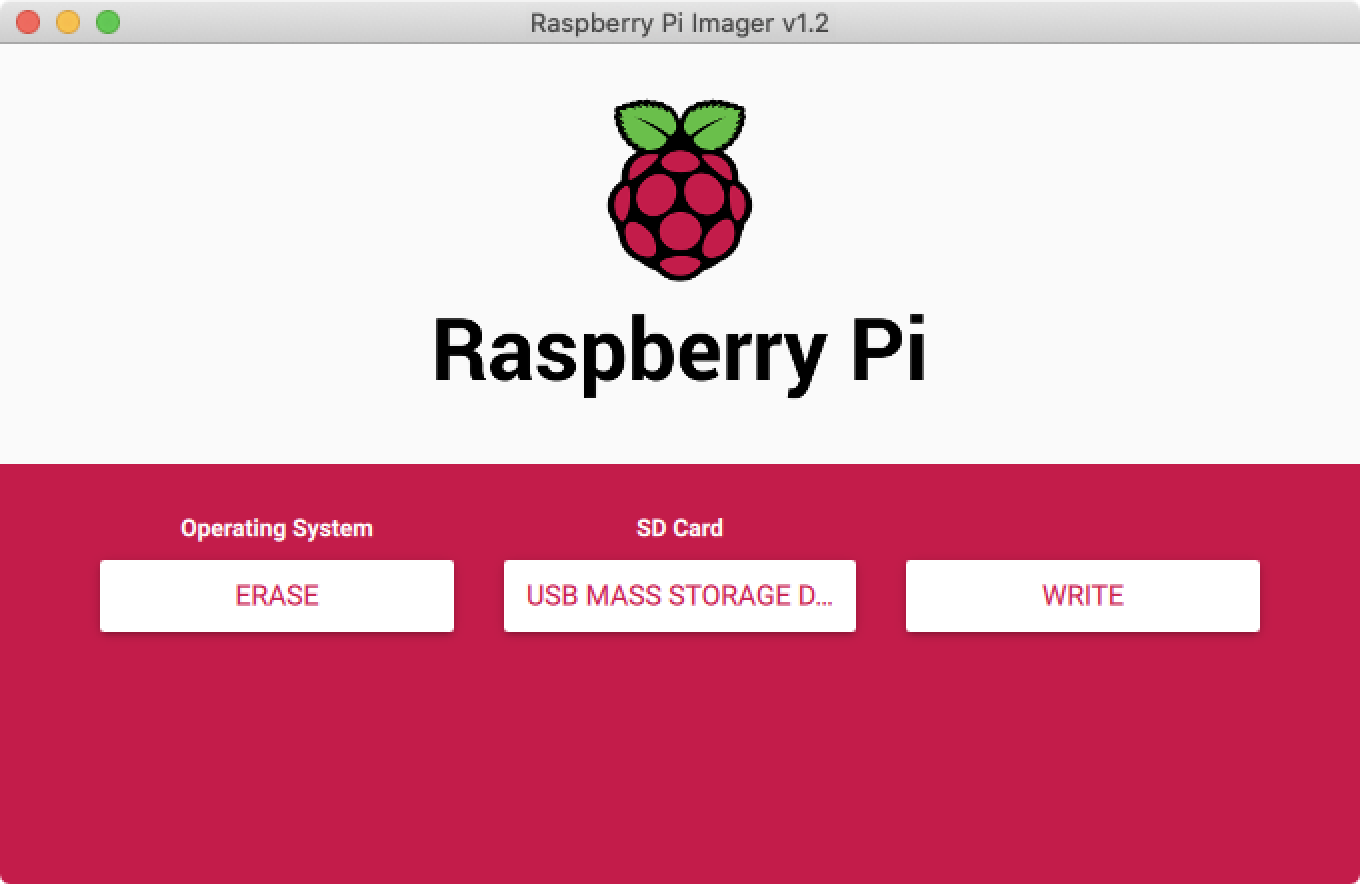
\includegraphics[width=1.0\textwidth]{screenshots/imager-erase.png}
	\caption{Using Raspberry Pi Imager to erase and format a MicroSD card.}
\end{figure}

Then use the Raspberry Pi Imager to write preinstalled server image to the MicroSD card...

\begin{figure}
	\centering	
	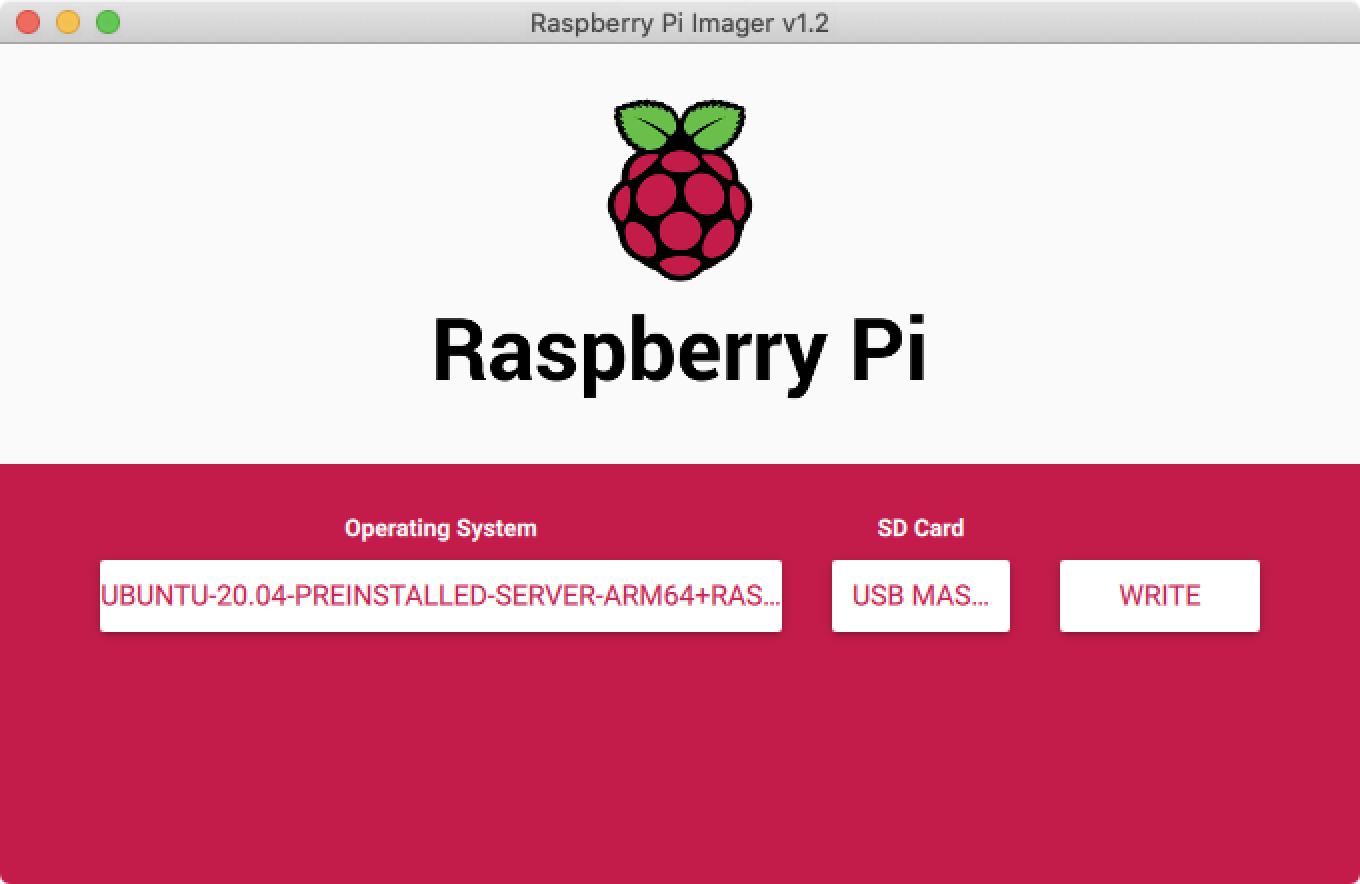
\includegraphics[width=1.0\textwidth]{screenshots/imager-write.png}
	\caption{Using Raspberry Pi Imager to write the server image to a MicroSD card.}
\end{figure}

When complete, remove the MicroSD card from the card reader, place it the Raspberry Pi and plug in the power cable.

The cloud-init configuration process will now start. The Raspberry Pi will acquire its IP address from the router, setup users, update apt, upgrade the system, download software packages, set the hostname (based on the IP address), and finally the system will reboot.


\subsection{Post-Installation Tasks}

\subsubsection{Enable No Password Access}

This is required for Open-MPI...

Our public key was installed on each node by cloud-init. So, we can ssh into each node without a password, and use the abbreviated ssh node1, instead of ssh john@node1 (assuming john is the user name on the workstation).

We need to copy our private key to node1 (only node1)...

\lstset{frameround=tttt}
\begin{lstlisting}[frame=single]
scp ~/.ssh/id_rsa node1:~/.ssh
\end{lstlisting}

Then to enable access to nodes node2 to node9 without a password from node1, we need to import the ... keys into the node1 knownhosts file...

This is easily done...

From macbook, ssh into node1...

ssh node1

and then from node1, for each of the nodes node2 to node9:

ssh node2

This will generate...

\lstset{frameround=tttt}
\begin{lstlisting}[frame=single]
The authenticity of host 'node2 (192.168.0.2)' can't be established.
ECDSA key fingerprint is SHA256:5VgsnN2nPvpfbJmALh3aJdOeT/NvDXqN8TCreQyNaFA.
Are you sure you want to continue connecting (yes/no/[fingerprint])?
\end{lstlisting}

responding yes, imports the key into the node1 knownhosts file...

\lstset{frameround=tttt}
\begin{lstlisting}[frame=single]
exit
\end{lstlisting}

Next node...

This is only required to be done on intial contact with nodes node2 to node9 (unless the keys on these nodes change)



\subsubsection{Uninstall unattended-upgrades}

The package unattended-upgrades is installed automatically...

Can potentially interferer with long running benchmarks...

Remove...

From macbookpro:

\lstset{frameround=tttt}
\begin{lstlisting}[frame=single]
ssh node1 sudo apt remove unattended-upgrades --yes
ssh node2 sudo apt remove unattended-upgrades --yes
ssh node3 sudo apt remove unattended-upgrades --yes
ssh node4 sudo apt remove unattended-upgrades --yes
ssh node5 sudo apt remove unattended-upgrades --yes
ssh node6 sudo apt remove unattended-upgrades --yes
ssh node7 sudo apt remove unattended-upgrades --yes
ssh node8 sudo apt remove unattended-upgrades --yes
ssh node9 sudo apt remove unattended-upgrades --yes
\end{lstlisting}

Don't forget to update your cluster regularly at convenient times...

See update/upgrade script below...



\subsubsection{Create a Project Repository}

Xpand upon...

\lstset{frameround=tttt}
\begin{lstlisting}[frame=single]
ssh node1
mkdir picluster
cd picluster
git init
\end{lstlisting}

Ensure you do  

git add
git commit
git push

at regular intervals...



\subsubsection{Create an System Update/Upgrade Script}

Automate...

\lstset{frameround=tttt}
\lstinputlisting[frame=single]{files/picluster-update}



\subsubsection{Select BLAS Library}

We have installed four BLAS libraries...

Confirm all nodes are using the same one initially...

ssh node1
sudo update-alternatives --config libblas.so.3-aarch64-linux-gnu

TODO screen output...

Confirm option 0, OpenBLAS, is selected. Press return to keep this option and then exit.



%
% APPENDIX B
%
\clearpage\section{Appendix B - High-Performance Linpack (HPL) Installation}

Download and install the latest version of HPL on node1...

\lstset{frameround=tttt}
\begin{lstlisting}[frame=single]
ssh node1
cd picluster
mkdir hpl
cd hpl
wget https://www.netlib.org/benchmark/hpl/hpl-2.3.tar.gz
gunzip hpl-2.3.tar.gz
tar xvf hpl-2.3.tar
rm hpl-2.3.tar
cd hpl-2.3
\end{lstlisting}

Create Make.serial file...

\lstset{frameround=tttt}
\begin{lstlisting}[frame=single]
cd setup
bash make_generic
cd ..
cp setup/Make.UNKNOWN Make.serial
\end{lstlisting}

Amend Make.serial as per...

Build...

\lstset{frameround=tttt}
\begin{lstlisting}[frame=single]
make arch=serial   
\end{lstlisting}

This creates xhpl and HPL.dat in bin/serial

Copy xhpl to all nodes (only xhpl, and not HPL.dat)...

\lstset{frameround=tttt}
\begin{lstlisting}[frame=single]
ssh node2 mkdir -p picluster/hpl/hpl-2.3/bin/serial
ssh node3 mkdir -p picluster/hpl/hpl-2.3/bin/serial
ssh node4 mkdir -p picluster/hpl/hpl-2.3/bin/serial
ssh node5 mkdir -p picluster/hpl/hpl-2.3/bin/serial
ssh node6 mkdir -p picluster/hpl/hpl-2.3/bin/serial
ssh node7 mkdir -p picluster/hpl/hpl-2.3/bin/serial
ssh node8 mkdir -p picluster/hpl/hpl-2.3/bin/serial
ssh node9 mkdir -p picluster/hpl/hpl-2.3/bin/serial

scp bin/serial/xhpl node2:~picluster/hpl/hpl-2.3/bin/serial
scp bin/serial/xhpl node3:~picluster/hpl/hpl-2.3/bin/serial
scp bin/serial/xhpl node4:~picluster/hpl/hpl-2.3/bin/serial
scp bin/serial/xhpl node5:~picluster/hpl/hpl-2.3/bin/serial
scp bin/serial/xhpl node6:~picluster/hpl/hpl-2.3/bin/serial
scp bin/serial/xhpl node7:~picluster/hpl/hpl-2.3/bin/serial
scp bin/serial/xhpl node8:~picluster/hpl/hpl-2.3/bin/serial
scp bin/serial/xhpl node9:~picluster/hpl/hpl-2.3/bin/serial
\end{lstlisting}



%
% APPENDIX C
%
\clearpage\section{Appendix D - Hints and Tips}

Hints from experience... and time savers... for building a development cluster on a local network.

% SUBSECTION
\subsection{IP/MAC Addresses}
If IP/MAC address assignments get confused, which is easily done during initial build, view IP address assignments on the local network with:

\begin{verbatim}
    arp -a
\end{verbatim}

Then delete \emph{incomplete} IP addresses with:

\begin{verbatim}
    sudo arp -d incomplete-ip-address
\end{verbatim}

% SUBSECTION
\subsection{SSH known\_hosts}
If \emph{ssh} reports differing keys in 'known-hosts', and warns of a potential 'man-in-the-middle-attack', then just delete 'known-hosts':

\begin{verbatim}
    sudo rm ~/.ssh/known_hosts
\end{verbatim}

'known\_hosts' will be re-populated as you log into each node. 


% SUBSECTION
\subsection{tmux}
\verb|tmux| is your friend!

Monitoring long running jobs from a workstation, which goes to sleep after a period of no activity, for example, may interfere with the running of the jobs if a SSH connection is broken.

Use a \verb|tmux| session to start long running jobs, and then detach from the \verb|tmux| session. The job will quite happily run in the background on the cluster. Turn the workstation off and go to bed. In the morning, turn the workstation on and 'attach' to the \verb|tmux| session. All will be well.

% SUBSECTION
\subsection{git}
\verb|git| is your best friend!

During your cluster build you will accidentally delete files, results etc. After every significant...


%
% APPENDIX - F
%
\clearpage\section{Appendix F - Pi Cluster Management Tools}

\lstinputlisting[frame=single, language=bash, numbers=left, caption=picluster/tools/picluster-update]{picluster/tools/picluster-update}
\lstinputlisting[frame=single, language=bash, numbers=left, caption=picluster/tools/picluster-reboot]{picluster/tools/picluster-reboot}
\lstinputlisting[frame=single, language=bash, numbers=left, caption=picluster/tools/picluster-shutdown]{picluster/tools/picluster-shutdown}
\lstinputlisting[frame=single, language=bash, numbers=left, caption=picluster/tools/picluster-libblas-query]{picluster/tools/picluster-libblas-query}
\lstinputlisting[frame=single, language=bash, numbers=left, caption=picluster/tools/picluster-libblas-set-openblas-serial]{picluster/tools/picluster-libblas-set-openblas-serial}
\lstinputlisting[frame=single, language=bash, numbers=left, caption=picluster/tools/picluster-libblas-set-openblas-openmp]{picluster/tools/picluster-libblas-set-openblas-openmp}
\lstinputlisting[frame=single, language=bash, numbers=left, caption=picluster/tools/picluster-libblas-set-blis-serial]{picluster/tools/picluster-libblas-set-blis-serial}
\lstinputlisting[frame=single, language=bash, numbers=left, caption=picluster/tools/picluster-libblas-set-blis-openmp]{picluster/tools/picluster-libblas-set-blis-openmp}

%
% THE END
%
\end{document}
